
Hardware selection was guided by the given requirements so that the control-tower prototype would operate as flawlessly and reliably as possible. It was also taken into account that the control tower should be as easy as possible to reconfigure for different vessel types. The requirements set for the system were:

\begin{itemize}
\item
  Three cameras as inputs, with a resolution of at least 1000$\times$1000 pixels.
\item
  Vessel-detection rate of at least 15 frames per second.
\end{itemize}

A similar system is intended to be applied to different vessel types in the future, so the components were chosen from among widely used and readily available devices.

\section{Control unit / onboard computer}\label{control-unit-onboard-computer}

The control unit is a device that processes information from the cameras attached to it and forwards the results to the autopilot. The onboard computer sits in the vessel's control tower, surrounded by three cameras. Analytical algorithms are applied to the information from the cameras (in this context, real-time video); their output -- detected objects and their relative positions in the frame -- is passed to the autopilot, providing additional information about the surrounding environment, on the basis of which the autopilot decides how the vessel should behave.

There are several single-board computers suitable for this task (\emph{Single-Board Computer}, SBC \cite{ref19}, \emph{System on Module} (SoM)), the most popular being the Nvidia Jetson series \cite{ref20}, which is specialised for AI, computer-vision, and machine-learning applications, and the Raspberry Pi \cite{ref21}. The Raspberry Pi is ruled out here because the control-tower system involves working with four cameras in parallel (the Raspberry Pi has only one camera input). The task requires substantial compute, but the Raspberry Pi lacks both the necessary throughput and the requisite hardware (the device's CPU does include an integrated graphics processor, but it is too weak for the task at hand). For parallel work, a discrete graphics processor (\emph{Graphics Processing Unit} (GPU) \cite{ref22}) together with specialised CUDA cores (\emph{CUDA Cores} \cite{ref23}) is particularly beneficial -- one of the Nvidia Jetson computers' main advantages.

The Jetson family contains four devices: Nano, TX2, Xavier NX, and AGX Xavier, the last of which is the most capable (see Table~\ref{tab:3-1-1}). The Nano is the most basic version, suitable for the simplest computer-vision applications; the TX2 is somewhat more capable in CPU and GPU performance; and the Xavier NX and AGX Xavier are aimed at industrial use cases, with six- and eight-core CPUs and Volta-architecture GPUs that also include matrix-operation accelerators (\emph{Tensor Cores}) \cite{ref24} (see Figure~\ref{fig:image7}).

\begin{longtable}[]{@{}
  >{\raggedright\arraybackslash}p{0.2297\linewidth}
  >{\raggedright\arraybackslash}p{0.2297\linewidth}
  >{\raggedright\arraybackslash}p{0.2568\linewidth}
  >{\raggedright\arraybackslash}p{0.2568\linewidth}@{}}
\caption{Parameters of the Jetson-series computers \cite{ref24}}\label{tab:3-1-1}\\
\toprule\noalign{}
\endhead
\bottomrule\noalign{}
\endlastfoot
\textbf{Parameters} & \textbf{Jetson
Nano} & \textbf{Jetson TX2
Series (NX,
TX2i)} & \textbf{Jetson Xavier
Series (NX,
AGX)} \\
AI Performance & 472 GFLOPs & 1.33 TFLOPs & 21/30 TOPs \\
GPU & 128-core
NVIDIA
Maxwell™ & 256-core NVIDIA
Pascal™ & 384/512-core
NVIDIA Volta™
with 48/64
Tensor Cores \\
CPU & Quad-Core Arm
Cortex-A57 & Dual-Core NVIDIA
Denver and
Quad-Core Arm
Cortex-A57 & 6/8-core NVIDIA
Carmel Arm \\
DL Accelerator & \begin{minipage}[t]{\linewidth}\raggedright
\begin{center}\rule{0.5\linewidth}{0.5pt}\end{center}
\end{minipage} & \begin{minipage}[t]{\linewidth}\raggedright
\begin{center}\rule{0.5\linewidth}{0.5pt}\end{center}
\end{minipage} & 2x NVDLA v1 \\
Vision
Accelerator & \begin{minipage}[t]{\linewidth}\raggedright
\begin{center}\rule{0.5\linewidth}{0.5pt}\end{center}
\end{minipage} & \begin{minipage}[t]{\linewidth}\raggedright
\begin{center}\rule{0.5\linewidth}{0.5pt}\end{center}
\end{minipage} & 2x PVA v1 \\
Memory & 4 GB

64-bit LPDDR4 & 4/8 GB

128-bit LPDDR4 & 8/16/32/64 GB

128-bit LPDDR4x \\
Storage & 16 GB & 16/32 GB & 16/35/64 GB \\
CSI Camera & Up to 4
cameras

(up to 18
Gbps) & \begin{minipage}[t]{\linewidth}\raggedright
Up to 5/6
cameras\\
(up to 30 Gbps)\strut
\end{minipage} & Up to 6 cameras

(up to 62 Gbps) \\
\end{longtable}

Given that information from three cameras must be analysed in parallel and with high accuracy, it makes the most sense to use a Xavier-series system. Compared with the other series, the Xavier-series computers offer their performance through a larger number of GPU cores, a newer architecture (Volta \cite{ref25}) that includes matrix accelerators (\emph{Tensor Cores}, which neural networks need for matrix computations), and Deep Learning Accelerators, which enable more efficient processing with multiple camera inputs.

Within this series both the NX and AGX Jetsons are available, and the best candidates have been chosen (see Table~\ref{tab:3-1-2}). The most suitable among these is the Jetson AGX Xavier, because the device must be able to run a large neural network and handle several operations at once (reading information from the cameras, processing it in the neural network, and presenting the processed information in the output video), which requires substantial computational resources.

\begin{longtable}[]{@{}
  >{\raggedright\arraybackslash}p{0.1944\linewidth}
  >{\raggedright\arraybackslash}p{0.3241\linewidth}
  >{\raggedright\arraybackslash}p{0.4630\linewidth}@{}}
\caption{Parameters of the Jetson AGX Xavier and the Xavier NX \cite{ref24}}\label{tab:3-1-2}\\
\toprule\noalign{}
\endhead
\bottomrule\noalign{}
\endlastfoot
\textbf{Parameters} & \textbf{Jetson AGX Xavier} & \textbf{Jetson Xavier NX 16GB} \\
AI Performance & 32 TOPs & 21 TOPs \\
GPU & \begin{minipage}[t]{\linewidth}\raggedright
512-core NVIDIA Volta™ GPU with\\
64 Tensor Cores\strut
\end{minipage} & 384-core NVIDIA Volta™ GPU with 48 Tensor Cores \\
CPU & \begin{minipage}[t]{\linewidth}\raggedright
8-core NVIDIA Carmel Arm®v8.2\\
64-bit CPU\\
8MB L2 + 4MB L3\strut
\end{minipage} & \begin{minipage}[t]{\linewidth}\raggedright
6-core NVIDIA Carmel Arm®v8.2 64-bit CPU\\
6MB L2 + 4MB L3\strut
\end{minipage} \\
DL Accelerator & 2x NVDLA v1 & 2x NVDLA v1 \\
Vision Accelerator & 2x PVA v1 & 2x PVA v1 \\
Memory & \begin{minipage}[t]{\linewidth}\raggedright
32 GB 256-bit LPDDR4x\\
136,5 GB/s\strut
\end{minipage} & \begin{minipage}[t]{\linewidth}\raggedright
16 GB 128-bit LPDDR4x\\
59,7 GB/s\strut
\end{minipage} \\
Storage & 32 GB eMMC 5.1 & 16 GB eMMC 5.1 \\
CSI Camera & Up to 6 cameras (up to 62 Gbps) & Up to 6 cameras (up to 30 Gbps) \\
\end{longtable}

\begin{figure}[H]
\centering
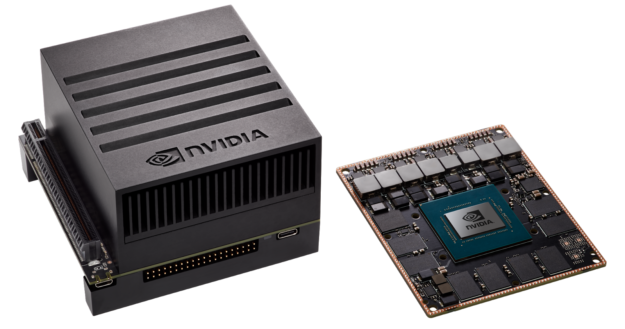
\includegraphics[width=4.09763in,height=2.08472in]{media/image7.png}
\caption{The chosen computer: the Jetson AGX Xavier (right, without the heat-sink module) \cite{ref26}}\label{fig:image7}
\end{figure}

\section{Tensor cores and CUDA}\label{tensor-cores-and-cuda}

Tensor Cores are programmable matrix-operation accelerators that perform their operations in parallel with the CUDA \cite{ref23} cores. These cores implement a newer kind of mixed-precision floating-point and integer operations -- HMMA (\emph{Half-Precision Matrix Multiply and Accumulate}) and IMMA (\emph{Integer Matrix Multiply and Accumulate}) -- which accelerate linear algebra, signal processing, and deep-learning inference \cite{ref27} (see Figure~\ref{fig:image8}).

\begin{figure}
\centering
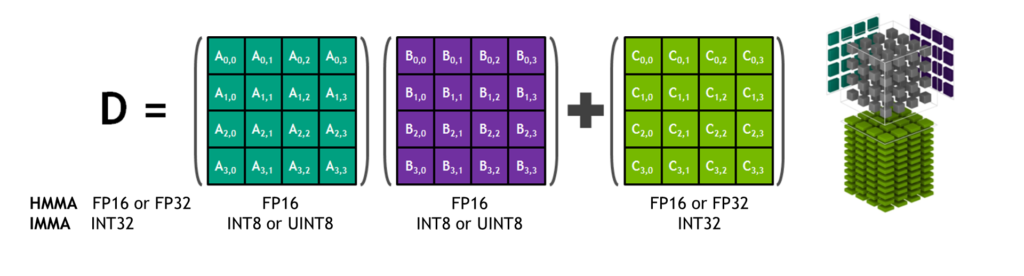
\includegraphics[width=6.10278in,height=1.64514in,alt={Jetson Xavier Tensor Core Matrix diagram}]{media/image8.png}
\caption{A Tensor Core multiplying and summing three-dimensional 4$\times$4$\times$4 matrices \cite{ref27}}\label{fig:image8}
\end{figure}

CUDA is a parallel-computing platform and programming model that increases the number of computations multi-fold by using the GPU in place of the CPU \cite{ref23}.

The purpose of CUDA is to accelerate parallel computation, and a CUDA core is analogous to a CPU core. The only difference is in their construction: a CPU core is able to solve complex computations sequentially, while a CUDA core handles simpler computations in the GPU. The GPU's advantage over the CPU is that thousands of CUDA cores are placed on a single chip, which allows complex computations to be divided among many cores and therefore performed faster than a CPU with a smaller number of more capable cores. This technology is integrated and widely used in the machine-learning field by Nvidia.

\section{Cameras}\label{cameras}

When selecting cameras, several parameters must be considered to ensure that the system meets the requirements and operates successfully. Because in this task the computer-vision system is housed in the control tower, which is mounted on the vessel's mast, the cameras (or the housing in which they are placed) must be capable of operating across wide temperature ranges and changing weather conditions. The camera software should also be chosen to favour the newest and clearly documented material, and its compatibility with the host computer must be considered. This ensures better camera configuration and makes the deployed computer-vision software easier to manage.

The following parameters were considered when selecting cameras:

\begin{itemize}
\tightlist
\item
  \textbf{Resolution} (in pixels, px) -- directly tied to object-detection accuracy and detection speed. The lower the resolution of the input given to the detection algorithm, the less accurate/less certain the neural network's prediction. In this case the detection process is faster, since the algorithm deals with a smaller amount of data and fewer computations, which ultimately improves inference speed.
\end{itemize}

\begin{quote}
At higher resolution, detection accuracy improves but inference speed decreases, because the amount of input data grows. A high-resolution photograph contains more information, which in turn allows the neural network to give more confident predictions.
\end{quote}

\begin{itemize}
\item
  \textbf{Frame rate} (\emph{Frames per second}, FPS) -- a parameter that describes the camera's information throughput, i.e.\ the ratio between the number of frames transmitted and the time. A high frame rate ensures a visually smoother data stream and easier tracking, and also reduces data loss. At a low frame rate, tracking an object and predicting its trajectory would be significantly more difficult, because the object's motion is visually intermittent and the accuracy of the neural network's predictions is harmed accordingly.
\item
  \textbf{Colour sensor} (monochromatic or polychromatic sensor) -- i.e., single-colour or multi-colour sensor. A monochromatic sensor suits environments where the colour contrast between the object and the environment is large, ensuring effective object detection. Since this is a monochromatic image, a single value is given per pixel, falling in a fixed range (typically 0$\dots$255 or 0.0$\dots$1.0).
\end{itemize}

\begin{quote}
A polychromatic sensor, on the other hand, suits environments where the contrast between background and object is not very large, or where object detection requires more information. With this kind of image transmission, three values are given as a matrix per pixel, the RGB (Red, Green, Blue) colours each in the range 0$\dots$255 or 0.0$\dots$1.0 (for example [255, 0, 255]). This transmission mode is three times as data-heavy as transmitting a monochromatic image, since three values are given per pixel.
\end{quote}

Devices that would meet the parameters mentioned above are listed below (see Table~\ref{tab:3-3-1}):

\begin{longtable}[]{@{}
  >{\raggedright\arraybackslash}p{0.1753\linewidth}
  >{\raggedright\arraybackslash}p{0.2371\linewidth}
  >{\raggedright\arraybackslash}p{0.1856\linewidth}
  >{\raggedright\arraybackslash}p{0.1134\linewidth}
  >{\raggedright\arraybackslash}p{0.1134\linewidth}
  >{\raggedright\arraybackslash}p{0.1340\linewidth}@{}}
\caption{Cameras matching the parameters}\label{tab:3-3-1}\\
\toprule\noalign{}
\endhead
\bottomrule\noalign{}
\endlastfoot
\textbf{Camera
name} & \textbf{Resolution (px)} & \textbf{Frame rate
(FPS)} & \multicolumn{2}{>{\raggedright\arraybackslash}p{0.2268\linewidth + 2\tabcolsep}}{%
\textbf{Operating temp.
(°C)}} & \textbf{Interface} \\
SurveilsQUAD --
Sony IMX290
System \cite{ref28} & 1920x1080 & 120 & -30 & 85 & CSI \\
OpenCV AI Kit:
OAK---D \cite{ref29} & 1280x800 (stereo)
4056x3040 (centre) & 120 (stereo)

60 (centre) & N/A & N/A & USB-C/PoE \\
OpenCV AI Kit:
OAK---1-PoE
\cite{ref30} & 4056x3040 & 60 & N/A & N/A & USB-C/PoE \\
Atlas IP67 7.1
MP Model
\cite{ref31} & 3208x2200 & 74 & -20 & 55 & PoE \\
Atlas IP67 2.8
MP Model
\cite{ref32} & 1936x1464 & 173 & -20 & 55 & PoE \\
Arducam 12MP
IMX477 \cite{ref33} & 4056x3040 & 60 & N/A & N/A & USB-C \\
Arducam
Fisheye Camera
\cite{ref34} & 2592×1944 & 30 & N/A & N/A & CSI and
Ethernet \\
\end{longtable}

*N/A -- data not available

At the time of writing, the SurveilsQUAD cameras were initially used, since they had been prepared in advance for the computer system, and the relevant software modifications for the Xavier had already been made by project parties at the Department of Computer Systems. The project under development at the time of writing was in its development phase, so the budget was limited; we therefore made do, at first, with cameras whose baseline capabilities sufficed for the experiments. During the control-tower design it became apparent that the placement of the chosen cameras was limited by their short cables, and the manufacturer did not supply longer cables for the units.

Therefore the Arducam Mini camera was chosen (see Figure~\ref{fig:image9}), connected to a Raspberry Pi and from there, via an Ethernet cable, to an Ethernet switch and ultimately to the Jetson Xavier. This also solved the cable-length issue, and it became possible to install the latest software on the Xavier, which the older cameras' outdated drivers did not support.

\begin{figure}[H]
\centering
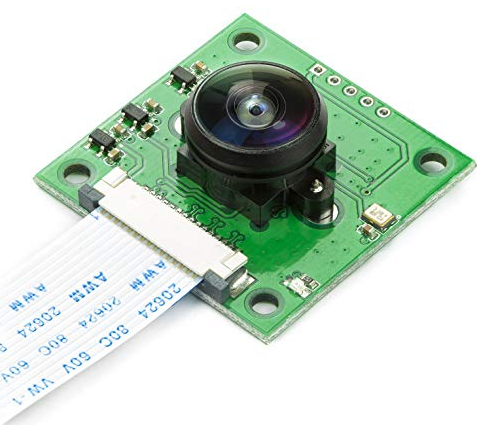
\includegraphics[width=2.75104in,height=2.42839in]{media/image9.png}
\caption{Module with the Arducam Fisheye camera \cite{ref34}}\label{fig:image9}
\end{figure}

\section{Control tower}\label{control-tower}

The control tower sits at the bow of the vessel (see Figure~\ref{fig:image11}) and its task is to take over control of the vessel on the captain's command and handle it autonomously with as little captain intervention as possible. To do this, the tower has a brain in the form of the Jetson AGX, which gathers information from all sensors and cameras, processes it, and then forwards a control decision to the autopilot, which in turn sends signals to the vessel's engines and rudder. The Jetson receives information about the surrounding environment from cameras, X-band radar, AIS, and a weather-station wind sensor. Data exchange within the control-tower system takes place via an Ethernet switch and a 4G router, which enables data to be sent and received from the user. Developers can also push software updates to the vessel's systems. AIS (Automatic Identification System) helps determine the vessel's position relative to other watercraft using satellites, the radar detects nearby objects as point clouds, and the cameras and the computer vision running on them identify vessels and other watercraft among the detected objects. AIS, radar, and the cameras with computer vision complement one another, helping the vessel detect and orient itself in its surroundings. The system is powered by a direct-current power source (see Figure~\ref{fig:image10}). 

\begin{figure}[H]
\centering
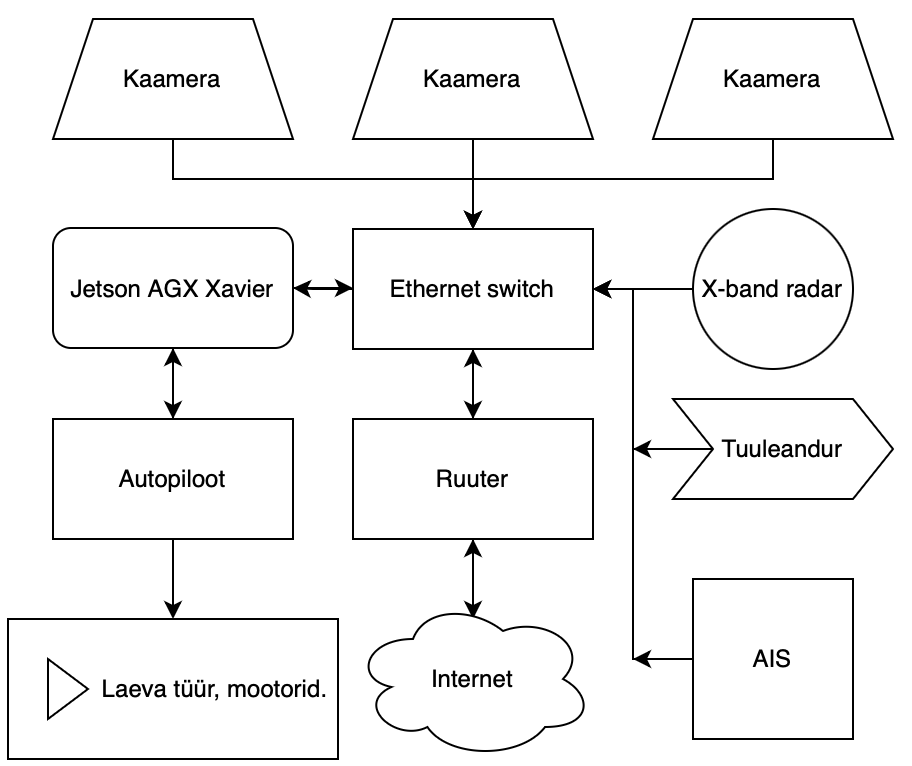
\includegraphics[width=6.10208in,height=5.125in]{media/image10.png}
\caption{Simplified operating diagram of the control tower}\label{fig:image10}
\end{figure}

\begin{figure}[H]
\centering
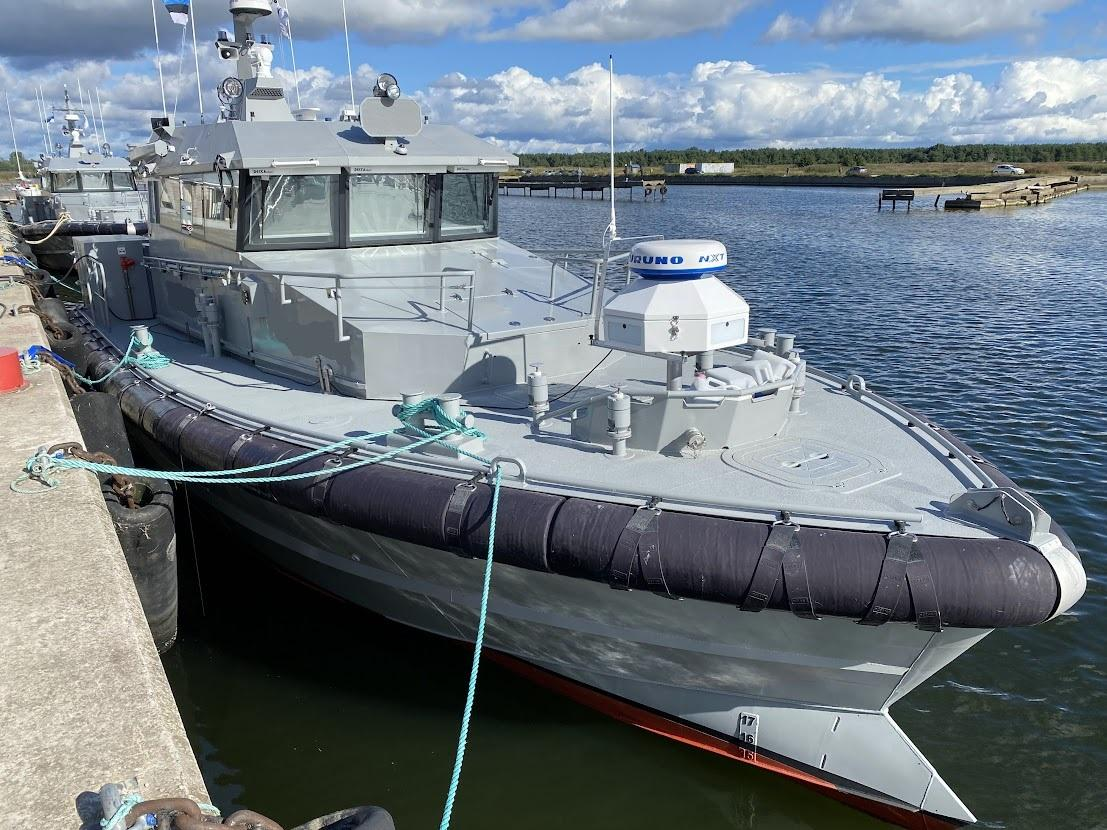
\includegraphics[width=6.10174in,height=4.56944in]{media/image11.jpg}
\caption{The control tower's placement on the patrol vessel \cite{ref35}}\label{fig:image11}
\end{figure}

